\graphicspath{{Skupina19/img/}}

\title{Primerjava disipacije energije reverzibilnih in ireverzibilnih polnih seštevalnikov v QCA}
\titlerunning{Reverzibilni polni seštevalniki v QCA}
\author{Denis Balant, Domen Breznik}
\maketitle

\abstract{Preverili smo, ali polni seštevalnik v QCA iz reverzibilnih vrat Torresa in sod. disipira manj energije kot ireverzibilni in zgolj logično reverzibilni seštevalniki. V orodju QCADesigner-E smo dve zgradbi seštevalnika izvedli s klasičnimi in s Torresovimi vrati ter ju pri periodah ure \SIlist{4;40;400}{\pico\second} primerjali še z dvema objavljenima zasnovama. Pri \SI{400}{ps} seštevalnika s Torresovimi vrati disipirata \num{10}- oziroma \num{20}-krat manj kot s klasičnimi vrati, najboljši doseže \num{1.3}\,$kT\ln 2$ na seštevanje, logično reverzibilen seštevalnik pa disipira toliko kot ireverzibilni.}

\section{Uvod}
\label{g19:sec:uvod}

Landauerjeva limita določa, da vsak izbrisan bit informacije stane vsaj $kT\ln 2$ energije~\cite{landauer1961}. Običajna logična vezja informacijo ves čas brišejo, saj iz izhodov logičnih vrat praviloma ni mogoče enolično rekonstruirati vhodov.

Kvantni celični avtomati (QCA) so ena od tehnologij, ki omogočajo reverzibilno procesiranje~\cite{lent1997}. Torres in sod.~\cite{g19:torres2019} so predlagali majoritetna vrata, ki poleg izhoda podajajo tudi kopije vhodov, in pokazali, da pri dovolj počasni uri disipirajo manj kot $kT\ln 2$ na operacijo. Takšna vrata imenujejo fizično reverzibilna. Ta definicija se razlikuje od tiste, ki smo jo spoznali pri predmetu, v tem delu pa jo uporabljamo, ker se nanaša na merljivo disipacijo.

Torres in sod. so iz svojih vrat sestavili le polovični seštevalnik, odvisnosti od hitrosti ure pa niso primerjali z drugimi zasnovami. Polni seštevalnik je osnovni gradnik aritmetičnih enot, ki ga v QCA običajno sestavimo iz treh majoritetnih vrat, na primer po zasnovi Wanga in sod.~\cite{g19:wang2003} ali Pudija in Sridharana~\cite{g19:pudi2012}. V literaturi nismo našli njegove izvedbe z vrati Torresa in sod. Za obe zasnovi smo sestavili lastni postavitvi, eno s klasičnimi majoritetnimi vrati in eno z vrati Torresa in sod., ter dobljene polne seštevalnike primerjali med seboj in z dvema objavljenima vezjema.

\begin{svgraybox}
\textbf{Raziskovalno vprašanje.}
Ali polni seštevalnik v QCA iz vrat Torresa in sod. disipira manj kot ireverzibilni in logično reverzibilni seštevalniki? Kako je to odvisno od hitrosti ure in kakšna je cena v številu celic, površini in zakasnitvi?
\textbf{Pričakovani rezultat.}
\begin{itemize}
    \item Pri zelo kratki urini periodi prevladujejo izgube zaradi hitrega preklapljanja celic, zato je disipacija približno sorazmerna s številom celic in reverzibilnost ne prinese bistvene prednosti.
    \item Pri počasnejši uri seštevalnik iz vrat Torresa in sod. disipira manj kot ostale izvedbe, ker vrata ne brišejo informacije, pri dovolj počasni uri pa celo manj od Landauerjeve limite. Pri ostalih zasnovah ostane cena brisanja, ki se s počasnejšo uro ne zmanjša.
    \item Zgolj logično reverzibilni seštevalnik disipira približno toliko kot ireverzibilni, ker njegova notranja vrata informacijo še vedno brišejo.
    \item Cena reverzibilnosti je več celic in večja zakasnitev.
\end{itemize}

\end{svgraybox}

\subsection{Osnove QCA}

Kvantni celični avtomati (angl.\ \textit{quantum-dot cellular automata}, QCA) predstavijo dvojiške podatke z razporeditvijo elektronov v celicah~\cite{lent1997}. Celico sestavljajo štiri kvantne pike in dva elektrona, ki se zaradi Coulombovega odboja razporedita v diagonalno nasprotni piki (slika~\ref{g19:fig:qca-celica}). Mogoči razporeditvi predstavljata polarizaciji $P = -1$ in $P = +1$ ter s tem logični vrednosti 0 in 1. Polarizacija celice vpliva na sosednje celice, zato lahko z ustrezno razporeditvijo celic prenašamo podatke in izvajamo logične operacije.

Smer in časovni potek prenosa določa ura, ki spreminja višino pregrad med pikami. Celice so razdeljene v urina območja, ki se v štirih fazah (preklop, zadrževanje, sproščanje, sproščenost) zaporedno polarizirajo, držijo stanje in ga izgubijo. Zaporedna območja so zamaknjena za četrtino periode, zato območje v fazi zadrževanja določa polarizacijo naslednjega območja v fazi preklopa.

\begin{figure}[H]
    \centering
    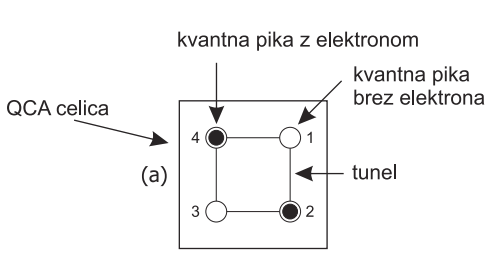
\includegraphics[width=0.50\linewidth]{qca_1.png}
    \caption{QCA celica}
    \label{g19:fig:qca-celica}
\end{figure}

\subsection{Logične strukture}
\label{g19:sec:strukture}

Najpreprostejša struktura QCA je vodilo, sestavljeno iz zaporedja sosednjih celic, po katerem se polarizacija vhodne celice prenese do izhoda (slika~\ref{g19:fig:gradniki}a). Z razvejitvijo vodila isti signal prenesemo na več mest v vezju, križanja vodil pa lahko izvedemo z več plastmi celic.

Osnovna gradnika za izvajanje logičnih operacij sta negator in majoritetna vrata. Negacijo dosežemo z diagonalno postavitvijo celic, pri kateri vhodna celica povzroči nasprotno polarizacijo izhodne (slika~\ref{g19:fig:gradniki}b). Trivhodna majoritetna vrata vrnejo vrednost, ki jo imata vsaj dva od treh vhodov:
\begin{equation}
M(A,B,C) = (A\land B)\lor(A\land C)\lor(B\land C).
\end{equation}
Klasična postavitev vsebuje tri vhodne celice, osrednjo celico in izhodno celico (slika~\ref{g19:fig:gradniki}c). Če en vhod nastavimo na konstantno vrednost, dobimo vrata IN oziroma ALI, $M(A,B,0) = A\land B$ in $M(A,B,1) = A\lor B$, zato majoritetna vrata in negator zadoščajo za poljubno dvojiško funkcijo.

\begin{figure}[H]
\centering
\begin{minipage}[b]{0.36\textwidth}\centering
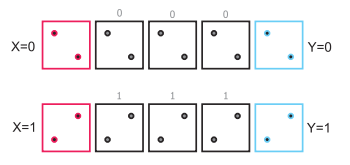
\includegraphics[width=\linewidth]{qca_vodilo.png}\\(a) vodilo
\end{minipage}\hfill
\begin{minipage}[b]{0.27\textwidth}\centering
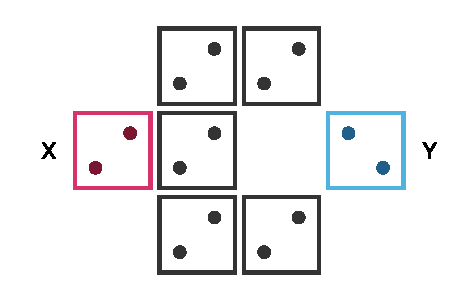
\includegraphics[width=\linewidth]{qca_negacija}\\(b) negator
\end{minipage}\hfill
\begin{minipage}[b]{0.30\textwidth}\centering
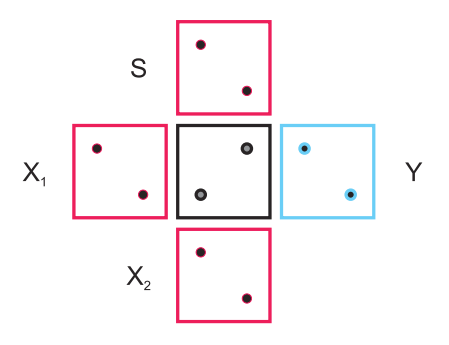
\includegraphics[width=\linewidth]{qca_majoritetna.png}\\(c) majoritetna vrata
\end{minipage}
\caption{Osnovni gradniki QCA.}
\label{g19:fig:gradniki}
\end{figure}


\subsection{Reverzibilne strukture}

Vezje je logično reverzibilno, če lahko iz izhodov enolično obnovimo vhode. Pri predmetu smo to definirali kot bijekcijo z enakim številom vhodov in izhodov. Majoritetna vrata tako niso reverzibilna, saj tri vhode preslikajo v en izhod. Vezja iz njih so lahko kot celota logično reverzibilna~\cite{g19:ahmad2018}, vendar informacijo znotraj vezja še vedno brišejo.

Vrata Torresa in sod.~\cite{g19:torres2019} (slika~\ref{g19:fig:torres}) poleg izhoda $f = M(A,B,C)$ posredujejo še kopije vhodov $A'$, $B'$ in $C'$. Njihova preslikava treh vhodov v štiri izhode ni bijekcija, je pa injektivna: vsakemu izhodu pripada največ en vhod. To zadošča, saj lahko injektivno preslikavo z dodatnim konstantnim vhodom dopolnimo v bijekcijo, entropija pa se pri njej ne spremeni, zato vrata informacije ne izgubijo~\cite{g19:torres2019}.

Torres in sod. svoja vrata imenujejo tudi fizično reverzibilna, ker disipirajo manj kot $kT\ln 2$ na operacijo. Te definicije se držimo v tem delu. Strožja definicija zahteva, da vezje deluje tudi v obratni smeri, torej da iz izhodov fizično izračuna vhode, česar ta vrata ne izpolnjujejo.

\begin{figure}[H]
\centering
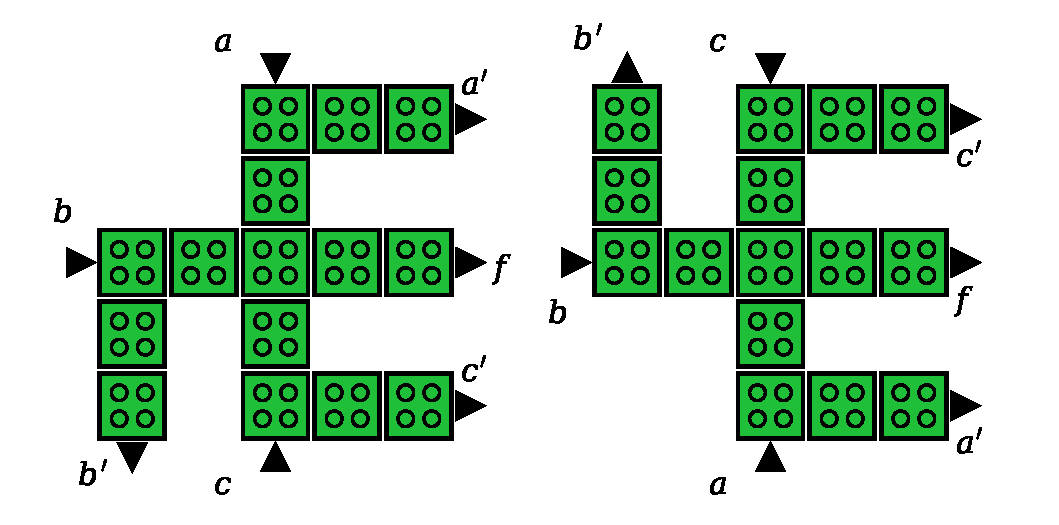
\includegraphics[width=0.85\textwidth]{torres_vrata}
\caption{Majoritetna vrata Torresa in sod. v dveh zrcalnih postavitvah: vhodi $a$, $b$, $c$, majoritetni izhod $f$ in kopije vhodov $a'$, $b'$, $c'$. Prirejeno po~\cite{g19:torres2019}.}
\label{g19:fig:torres}
\end{figure}

\subsection{Enobitni polni seštevalnik}

Enobitni polni seštevalnik je logično vezje, ki sešteje tri bite: $A$, $B$ in vhodni prenos $C_\mathrm{in}$. Rezultat sestavljata bit vsote $Sum$ in izhodni prenos $C_\mathrm{out}$ po izračunu
\begin{align}
    S &= A\oplus B\oplus C_\mathrm{in},\\
    C_\mathrm{out} &= (A\land B)\lor(A\land C_\mathrm{in})\lor(B\land C_\mathrm{in}).
\end{align}
Vsota je torej enaka $1$, kadar je število vhodnih enic liho, izhodni prenos pa je enak $1$, kadar sta vsaj dva vhoda enaka $1$, kar ustreza majoritetni funkciji. Vse kombinacije vhodov in izhodov prikazuje tabela~\ref{g19:tab:polni-sestevalnik}.

\begin{table}[H]
\centering
\caption{Pravilnostna tabela enobitnega polnega seštevalnika.}
\label{g19:tab:polni-sestevalnik}
\begin{tabular}{ccc|cc}
\hline
$A$ & $B$ & $C_\mathrm{in}$ & $S$ & $C_\mathrm{out}$ \\
\hline
0 & 0 & 0 & 0 & 0 \\
0 & 0 & 1 & 1 & 0 \\
0 & 1 & 0 & 1 & 0 \\
0 & 1 & 1 & 0 & 1 \\
1 & 0 & 0 & 1 & 0 \\
1 & 0 & 1 & 0 & 1 \\
1 & 1 & 0 & 0 & 1 \\
1 & 1 & 1 & 1 & 1 \\
\hline
\end{tabular}
\end{table}

\section{Metode}
\label{g19:sec:metode}

\subsection{Orodja in nastavitve}
\label{g19:sec:orodja}

Vezja smo načrtovali in simulirali v orodju QCADesigner-E~\cite{silltorres2018}, razširitvi orodja QCADesigner~\cite{walus2004}, ki simulatorju doda izračun disipirane energije vezja.

Uporabili smo privzete nastavitve koherenčnega simulatorja (tabela~\ref{g19:tab:nastavitve}), spreminjali smo le periodo ure in od nje odvisne parametre. Torres in sod.~\cite{g19:torres2019} so namreč pokazali, da je disipacija njihovih vrat močno odvisna od hitrosti ure, zato smo vezja simulirali pri periodah \SIlist{4;40;400}{\pico\second}.

\begin{table}[H]
\centering
\caption{Uporabljeni parametri simulacije v QCADesigner-E.}
\label{g19:tab:nastavitve}
\small
\begin{tabular}{ll}
\hline
Parameter & Vrednost \\
\hline
Temperatura & \SI{1}{\kelvin} \\
Čas relaksacije & \SI{e-15}{\second} \\
Perioda ure (= perioda vhodov) & \SIlist[list-units=single]{4;40;400}{\pico\second} \\
Časovni korak & \SI{e-16}{\second} \\
Čas simulacije & 12,5 urinih period (\SIlist[list-units=single]{0.05;0.5;5}{\nano\second})\\ 
Ura: visoka / nizka raven & \SI{9.8e-22}{\joule} / \SI{3.8e-23}{\joule} \\
Strmina ure (\textit{clock slope}) & četrtina periode (\SIlist[list-units=single]{1;10;100}{\pico\second}) \\
Relativna dielektričnost (\textit{permittivity}) & \num{12.9} \\
Polmer interakcije & \SI{80}{\nano\metre} \\
Razmik med plastmi & \SI{11.5}{\nano\metre} \\
\hline
Velikost celice / razmik celic & \SI{18}{\nano\metre} / \SI{20}{\nano\metre} \\
Premer pike & \SI{5}{\nano\metre} \\
\hline
\end{tabular}
\end{table}

S periodo smo sorazmerno spreminjali še strmino ure, periodo vhodov in skupni čas simulacije. Strmino, ki določa, kako hitro celice preklapljajo, smo nastavili na četrtino periode (\SIlist[list-units=single]{1;10;100}{\pico\second}). Perioda vhodov je enaka periodi ure, tako da se vhodi spremenijo enkrat na periodo ure in po vrsti zavzamejo vseh osem kombinacij $(A, B, C_\mathrm{in})$. Ena urina perioda tako ustreza enemu seštevanju. Skupni čas simulacije je 12,5 urinih period (\SIlist[list-units=single]{0.05;0.5;5}{\nano\second}), da povprečje pri vseh periodah zajame enako število ciklov.


Za disipirano energijo smo uporabili vrednost \textit{Avg\_Ebath}, ki jo izpiše QCADesigner-E: povprečno energijo, oddano v okolje v eni urini periodi, sešteto po vseh celicah, razen vhodnih, konstantnih in tistih, označenih z \textit{ignore\_energy}.

\subsection{Zasnova poskusov}
\label{g19:sec:poskusi}

Primerjali smo dve izvedbi polnega seštevalnika z majoritetnimi vrati, prikazani na sliki~\ref{g19:fig:sheme}.

\begin{figure}[H]
\centering
\begin{minipage}[b]{0.49\textwidth}\centering
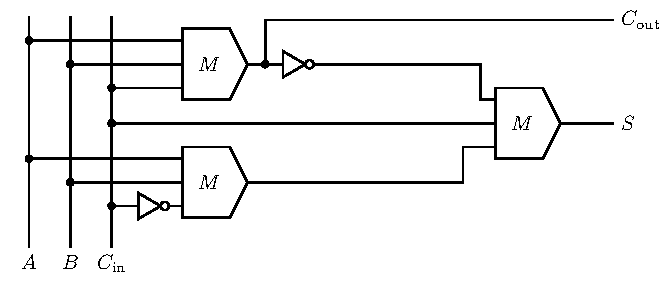
\includegraphics[width=\linewidth]{wang}\\[2pt](a) Wang in sod.~\cite{g19:wang2003}
\end{minipage}\hfill
\begin{minipage}[b]{0.49\textwidth}\centering
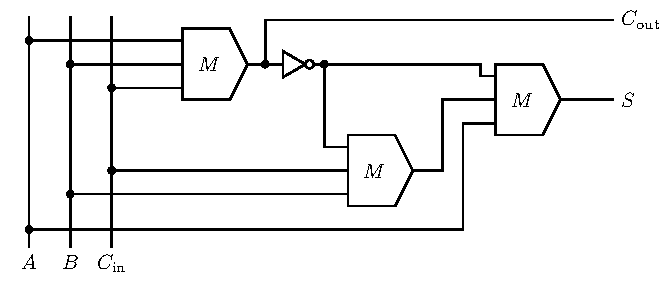
\includegraphics[width=\linewidth]{pudi}\\[2pt](b) Pudi in Sridharan~\cite{g19:pudi2012}
\end{minipage}
\caption{Logični shemi obeh izvedb polnega seštevalnika s tremi majoritetnimi vrati ($M$).}
\label{g19:fig:sheme}
\end{figure}

Wang in sod.~\cite{g19:wang2003} vmesna rezultata izračunajo vzporedno in potrebujejo tri majoritetna vrata in dva negatorja:

\begin{align}
C_\mathrm{out} &= M(A, B, C_\mathrm{in}),\\
S &= M(C_\mathrm{in}, \overline{C_\mathrm{out}}, M(A, B, \overline{C_\mathrm{in}})).
\end{align}

Pudi in Sridharan~\cite{g19:pudi2012} vrata povežeta zaporedno in se tako izogneta enemu negatorju:

\begin{align}
C_\mathrm{out} &= M(A, B, C_\mathrm{in}),\\
S &= M(\overline{C_\mathrm{out}}, M(C_\mathrm{in}, \overline{C_\mathrm{out}}, B), A).
\end{align}

V naši postavitvi smo $C_\mathrm{out}$ dobili z negacijo $\overline{C_\mathrm{out}}$, da smo se izognili križanju, zato ima tudi ta izvedba dva negatorja.

Obe izvedbi smo izdelali s klasičnimi majoritetnimi vrati in z vrati Torresa in sod.~\cite{g19:torres2019}. Tako smo dobili štiri vezja (slika~\ref{g19:fig:vezja-maj}).

\begin{figure}[H]
\centering
\begin{tabular}{@{}cc@{}}
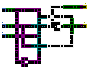
\includegraphics[width=0.58\textwidth]{wang_irr} &
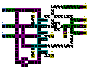
\includegraphics[width=0.58\textwidth]{wang_torres} \\
(a) Wang in sod.~\cite{g19:wang2003}, klasična vrata & (b) Wang in sod.~\cite{g19:wang2003}, vrata Torresa in sod. \\[6pt]
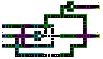
\includegraphics[width=0.58\textwidth]{pudi_irr} &

\includegraphics[width=0.58\textwidth]{pudi_torres} \\
(c) Pudi in Sridharan~\cite{g19:pudi2012}, klasična vrata & (d) Pudi in Sridharan~\cite{g19:pudi2012}, vrata Torresa in sod. \\
\end{tabular}
\caption{Postavitve polnih seštevalnikov v orodju QCADesigner-E po logičnih shemah Wanga in sod.~\cite{g19:wang2003} (a, b) ter Pudija in Sridharana~\cite{g19:pudi2012} (c, d). (a) in (c) sta izvedbi s klasičnimi majoritetnimi vrati, (b) in (d) pa izvedbi z reverzibilnimi vrati Torresa in sod.~\cite{g19:torres2019} in dodatnimi pomnilnimi izhodi.}
\label{g19:fig:vezja-maj}
\end{figure}

Za primerjavo z objavljenimi zasnovami smo po slikah iz člankov ponovno izdelali še dve vezji, ki ne sledita zgradbi s konvencionalnimi majoritetnimi vrati (slika~\ref{g19:fig:vezja-nemaj}).

Ahmad in sod.~\cite{g19:ahmad2018} predlagajo dvoje novih reverzibilnih vrat (3$\times$3-NRG in modificirana Feynmanova vrata) in iz njih sestavijo enoplastni logično reverzibilni seštevalnik-odštevalnik.

Seyedi in Jafari Navimipour~\cite{g19:seyedi2022} uporabita nova trivhodna majoritetna vrata, katerih vhodi so v različnih plasteh, ter vrata TIEO (\textit{angl. Three input exclusive-or gate}), in iz njih sestavita ireverzibilni seštevalnik v treh plasteh.

\begin{figure}[H]
\centering
\begin{tabular}{@{}cc@{}}

\includegraphics[width=0.58\textwidth]{ahmad2018.pdf} &

\includegraphics[width=0.48\textwidth]{seyedi.pdf} \\
(a) Ahmad in sod.~\cite{g19:ahmad2018} & (b) Seyedi in J.~N.~\cite{g19:seyedi2022} \\[6pt]
\end{tabular}
\caption{Postavitvi vezij, rekonstruirani po objavljenih zasnovah v orodju QCADesigner-E: (a) enoplastni logično reverzibilni seštevalnik-odštevalnik Ahmada in sod.~\cite{g19:ahmad2018}. (b) triplastni ireverzibilni polni seštevalnik Seyedija in Jafarija Navimipourja~\cite{g19:seyedi2022}.}
\label{g19:fig:vezja-nemaj}
\end{figure}

Vse štiri postavitve smo načrtovali ad hoc po logičnih shemah. Urina območja smo dodelili v navpičnih pasovih, tako da signal teče od leve proti desni in vsak pas pripada eni urini coni. Uporabili smo triplastno križanje, kjer se signal po navpičnih celicah dvigne v drugo plast celic in se za križanjem vrne v glavno plast.

Pri vratih Torresa in sod. smo razporeditev con povzeli po njihovih slikah: vrata so v svoji coni, dodatni izhodi pa so zaključeni s kratkimi vodili. Po njihovem vzorcu smo pri vseh šestih vezjih z \textit{ignore\_energy} označili celice vhodnih vodil do prvih vrat in celice izhodnih vodil od zadnjih vrat do izhodov, pri vezjih s Torresovimi vrati pa tudi celice dodatnih izhodov. Energija teh celic zato ni vključena v rezultate. Vsa vezja smo simulirali pri periodah \SIlist{4;40;400}{\pico\second}.

\subsection{Metrike}
\label{g19:sec:metrike}

Opisana vezja smo primerjali z naslednjimi metrikami:

\begin{itemize}
    \item število celic, površina, število križanj, zakasnitev v urinih ciklih,
    \item disipacija energije na celico in razmerje do Landauerjeve limite,
    \item pravilnost vseh izhodov in najmanjša absolutna polarizacija izhodov,
    \item število nepotrebnih (pomnilnih) izhodov.
\end{itemize}
 
\section{Rezultati}
\label{g19:sec:rezultati}

Vsa vezja so pri vseh treh periodah ure pravilno izračunala $S$ in $C_\mathrm{out}$ za vse vhodne vektorje. Lastnosti posameznih implementacij so zbrane v tabeli~\ref{g19:tab:cena}. Uporaba vrat Torresa in sod. namesto majoritetnih vrat poveča število celic za \SI{12}{\percent} (Pudi) oziroma \SI{20}{\percent} (Wang) in doda pet oziroma sedem dodatnih izhodov, najmanjša absolutna polarizacija celic se ne spremeni, površina in zakasnitev vezja pa se ne povečata.

\begin{table}[H]
\centering
\caption{Lastnosti implementacij. Celice vključujejo vhodne in izhodne celice, štete celice so celice, ki jih upoštevamo pri energiji (brez vhodnih, konstantnih in izhodnih celic). Površina je očrtani pravokotnik ene plasti, zakasnitev je število urinih con od vhoda do izhoda, deljeno s 4. Dodatni izhodi so izhodi poleg $S$ in $C_\mathrm{out}$.}
\label{g19:tab:cena}
\small
\setlength{\tabcolsep}{4pt}
\begin{tabular}{l S[table-format=3.0] S[table-format=3.0] S[table-format=1.3] c S[table-format=1.2] c S[table-format=1.2]}
\hline
Vezje & {Celice} & {Štete} & {Površina} & {Križanja} & {Zakasnitev} & {Dodatni} & {min $|P|$} \\
 & & {celice} & {[\si{\micro\metre\squared}]} & & {[cikli]} & {izhodi} & \\
\hline
Pudi (klasična) & 153 & 131 & 0.202 & 2 & 1.75 & 0 & 0.95 \\
Pudi (Torres)   & 171 & 145 & 0.189 & 4 & 1.75 & 5 & 0.95 \\
Wang (klasična) & 157 & 141 & 0.196 & 3 & 1.50 & 0 & 0.95 \\
Wang (Torres)   & 187 & 157 & 0.196 & 3 & 1.50 & 7 & 0.95 \\
\hline
Ahmad in sod.   & 121 & 103 & 0.143 & 0 & 1.25 & 3 & 0.95 \\
Seyedi in J.~N. &  18 &  12 & 0.014 & 0\rlap{$^\ast$} & 0.50 & 0 & 0.71 \\
\hline
\multicolumn{8}{l}{\footnotesize $^\ast$ tri plasti celic brez križanj, površina je površina ene plasti.}
\end{tabular}
\end{table}

Disipirane energije opisanih vezij so zbrane v tabeli~\ref{g19:tab:energija}, njihovo spreminjanje s periodo ure pa prikazuje slika~\ref{g19:fig:energija}.

Pri \SI{4}{ps} vsa večja vezja disipirajo med \num{2.9} in \SI{4.5}{\milli\electronvolt} na seštevanje, vezje Seyedija in J.~N. pa \SI{0.76}{\milli\electronvolt}. Pri \SI{400}{ps} se izvedbi s Torresovimi vrati zmanjšata na \SI{0.093}{\milli\electronvolt} (Pudi) in \SI{0.080}{\milli\electronvolt} (Wang), kar je \num{1.6}- oziroma \num{1.3}-kratnik Landauerjeve limite ($kT\ln 2$) in manj kot \SI{1}{\micro\electronvolt} na celico. Ostala vezja pri tej periodi disipirajo od \num{0.62} do \SI{1.66}{\milli\electronvolt}, kar je \num{10}- do \num{28}-kratnik $kT\ln 2$. Nobeno vezje ne pade pod Landauerjevo limito na operacijo, ki jo kot merilo uporabljajo tudi Torres in sod.~\cite{g19:torres2019}.

\begin{table}[H]
\centering
\caption{Disipirana energija na seštevanje (\textit{Avg\_Ebath}) pri treh periodah ure in pri \SI{400}{ps} še na celico in v enotah $kT\ln 2 = \SI{0.0597}{\milli\electronvolt}$. Energija na celico je izračunana glede na celice, ki niso označene z \textit{ignore\_energy}.}
\label{g19:tab:energija}
\small
\setlength{\tabcolsep}{4pt}
\begin{tabular}{l S[table-format=1.3] S[table-format=1.3] S[table-format=1.3] S[table-format=2.2] S[table-format=2.1]}
\hline
Vezje & \multicolumn{3}{c}{$E$ [\si{\milli\electronvolt}]} & \multicolumn{2}{c}{pri \SI{400}{ps}} \\
 & {\SI{4}{ps}} & {\SI{40}{ps}} & {\SI{400}{ps}} & {na celico [\si{\micro\electronvolt}]} & {$E/kT\ln 2$} \\
\hline
Pudi (klasična) & 3.40 & 1.16 & 0.94  & 7.19 & 15.8 \\
Pudi (Torres)   & 2.87 & 0.34 & 0.093 &  0.64 &  1.6 \\
Wang (klasična) & 4.49 & 1.85 & 1.59  & 11.27 & 26.6 \\
Wang (Torres)   & 3.33 & 0.37 & 0.080 &  0.51 &  1.3 \\
\hline
Ahmad in sod.~\cite{g19:ahmad2018}   & 3.29 & 1.79 & 1.66  & 16.11 & 27.8 \\
Seyedi in J.~N.~\cite{g19:seyedi2022} & 0.76 & 0.64 & 0.62  & 51.75 & 10.4 \\
\hline
\end{tabular}
\end{table}

\begin{figure}[H]
\centering
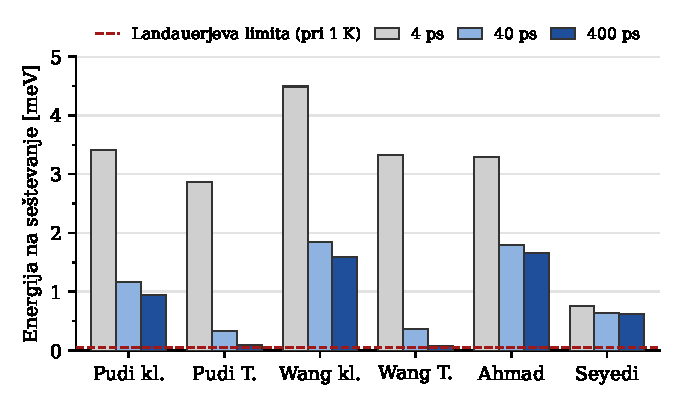
\includegraphics[width=\textwidth]{fig_energija}
\caption{Disipirana energija na seštevanje (\textit{Avg\_Ebath}) pri treh periodah ure. Kl. pomeni klasična majoritetna vrata, T. pomeni vrata Torresa in sod. Črtkana črta je Landauerjeva limita ($kT\ln 2 = \SI{0.0597}{\milli\electronvolt}$ pri \SI{1}{\kelvin}).}
\label{g19:fig:energija}
\end{figure}


% glede na metrike tabela + graf + poves v besedah kaj je na grafu  (1 stran)

% \section{Razprava}
% \label{g19:sec:razprava}

% govoris / obrazlozitev o ugotovitvah / rezultatih

% \subsection{Kaj ni delovalo}
% \label{g19:sec:neuspehi}

% ???

\section{Razprava}
\label{g19:sec:razprava}

Pričakovali smo, da bo pri kratki urini periodi disipacija naraščala z velikostjo vezja in da reverzibilnost ne bo prinesla bistvene prednosti. Rezultati to potrjujejo: pri \SI{4}{ps} večja vezja disipirajo od \num{2.9} do \SI{4.5}{\milli\electronvolt}, desetkrat manjše vezje Seyedija in J.~N. pa približno petkrat manj. Torresova vrata v tem območju prinesejo le od \num{16} do \SI{26}{\percent} prihranka.
 
Njihova prednost postane izrazita šele pri počasnejši uri. Med \SI{40}{ps} in \SI{400}{ps} se disipacija izvedb s Torresovimi vrati zmanjša za \num{73} do \SI{79}{\percent}, pri ostalih pa le za \num{3} do \SI{19}{\percent}, saj še vedno plačujejo energijsko ceno brisanja informacije~\cite{landauer1961,g19:torres2019}. Pri \SI{400}{ps} disipirata izvedbi Pudijevega in Wangovega seštevalnika s temi vrati \num{10}-krat oziroma \num{20}-krat manj kot ustrezni izvedbi s klasičnimi vrati. Kljub temu hipoteze, da bo celoten seštevalnik padel pod Landauerjevo limito, nismo potrdili. Najboljši rezultat doseže Wangova zasnova z \num{1.3}\,$kT\ln 2$ na seštevanje.

Tudi zgolj logična reverzibilnost ne zagotavlja bistveno manjše disipacije. Ahmadovo vezje~\cite{g19:ahmad2018} se med \SI{4}{ps} in \SI{400}{ps} izboljša le za faktor \num{2}, pri najdaljši periodi pa disipira toliko kot Wangova izvedba s klasičnimi vrati. Razlog je v ireverzibilnosti njegovih notranjih vrat. Čeprav Torresova vrata zahtevajo od \num{12} do \SI{20}{\percent} več celic in pet oziroma sedem dodatnih izhodov, pričakovanega povečanja zakasnitve nismo opazili.

Rezultati so iz simulacije v enem orodju pri enem naboru parametrov, postavitve pa niso optimizirane. Meritve energije ne vključujejo izgub na vhodu in izhodu. Težave z brisanjem signalov tako niso odpravljene, ampak samo prenesene na izhod. Dodatne izhode (pomnilne linije) bi bilo treba v večjem vezju uporabiti za nadaljnje računanje ali izbrisati, kar bi zahtevalo dodatno energijo.


\subsection{Kaj ni delovalo}
\label{g19:sec:neuspehi}

Pri prvih postavitvah se je izkazalo, da nekateri preprosti gradniki v večjem vezju niso zanesljivi. Dodatni izhodi, ki so se končali z eno samo celico, niso bili stabilni, zato smo jih podaljšali na dve celici. Dvoplastna križanja so motila sosednje celice, zato smo uporabili triplastna, preprosti negator z eno diagonalno celico pa smo nadomestili z robustnejšo izvedbo z dvema vejama. Preizkusili smo tudi strožjo definicijo fizične reverzibilnosti, vendar vrata Torresa in sod. v obratni smeri vhodov niso pravilno obnovila, kadar je bil obnovljeni vhod v manjšini.

\section{Zaključek}
\label{g19:sec:zakljucek}

Z vrati Torresa in sod. smo implementirali dva polna seštevalnika v QCA, po zgradbi Wanga in sod. ter Pudija in Sridharana, in ju primerjali z enakima seštevalnikoma s klasičnimi majoritetnimi vrati ter z dvema objavljenima zasnovama. Pri periodi ure \SI{4}{ps} so vsi seštevalniki disipirali približno sorazmerno z njihovo velikostjo, saj prevladujejo izgube zaradi hitrega preklapljanja. Pri \SI{400}{ps} sta seštevalnika s Torresovimi vrati disipirala \num{10}- oziroma \num{20}-krat manj kot s klasičnimi vrati, za ceno \num{12} do \SI{20}{\percent} več celic, brez večje površine ali zakasnitve. Logično reverzibilen seštevalnik Ahmada in sod. je disipiral približno toliko kot ireverzibilna, kar potrjuje, da logična reverzibilnost brez reverzibilnih notranjih vrat ne zadošča. Najboljši seštevalnik je dosegel \num{1.3}\,$kT\ln 2$ na seštevanje in se Landauerjevi limiti močno približal, a je ni presegel.

V nadaljnjem delu bi bilo smiselno raziskati, kako dodatne izhode uporabiti ali odstraniti v večjem vezju, na primer večbitnem seštevalniku, ne da bi s tem izgubili prihranek energije. Zanimivo bi bilo tudi preveriti, ali bi bilo mogoče uporabiti vrata, ki bi delovala tudi v obratni smeri in s tem izpolnjevala strožjo definicijo fizične reverzibilnosti ter tako morda zagotovila še večji prihranek energije.

\section*{Doprinosi avtorjev}

Denis Balant je načrtoval seštevalnika z vrati Torresa in sod. in napisal poglavja o osnovah QCA, logičnih in reverzibilnih strukturah. Domen Breznik je načrtoval seštevalnika s klasičnimi majoritetnimi vrati, ponovno izdelal objavljeni zasnovi in napisal uvod. Simulacije, analizo rezultatov, razpravo in zaključek sva pripravila skupaj.

\section*{Izjava o uporabi generativne umetne inteligence}

Pri delu sva si pomagala z jezikovnim modelom Claude Opus 5.5. Pomagal nama je pri interpretaciji rezultatov, pri iskanju in preverjanju literature ter pri pripravi tabel, slik in jezikovnem urejanju besedila v \LaTeX{}.
